\taughtsession{Lecture}{A8: Application of context-free grammars}{2025-10-20}{15:00}{Janka}

The idea of a context-free language was first proposed in the mid 1950s by Chomsky. The idea was to describe the grammar of English in terms of their block structure, and recursively built up from smaller phrases. An essential property of these block structures is that the logical units never overlap.

An example, as seen below, shows how a sentence can be comprised of three blocks:
\begin{center}
    ``((The boy touches) (the other boy (with the flower.)))''
\end{center}

Whilst context-free grammars are simple and mathematically precise, the derivations can add some ambiguity. For example, taking the above sentence - there are at least two possible interpretations of it: one boy uses the flower to touch the other boy; or one boy touches the other boy who is holding the flowers. The ambiguity is introduced because the same string can be derived in multiple ways; so to understand the true meaning of the string - we must understand the way in which it was derived.

\section{Derivations and Parse Trees}
\begin{define}
    \item[Parse Tree] is a diagrammatic representation of the parsed structure of a sentence or string.
\end{define}

Parse trees can be used to describe a derivation, starting with an initial symbol and working down towards the string.

The start symbol of a set of production rules is the tree's root. The tree is built by adding children to the nodes in the tree; for a production $X \rightarrow Y_1 \ldots Y_n$ children $Y_1, \ldots, Y_n$ are added to the tree. Terminals are added at the leaves, non-terminals at the interior nodes.

\begin{example}{Parse Trees}
If we consider a grammar fragment for simple arithmetic expressions where $E$ is the only non-terminal:
\[E \rightarrow E - E\ |\ 0\ |\ 1\ |\ 2\ |\ 4\ |\ 5\ |\ 6\ |\ 7\ |\ 8\ |\ 9\]

We can derive strings such as $4-8$, $9-1$, $5-6-9-2$, etc. We can also assign a meaning (or value, in this case) to the strings: $4-8=-4$, $9-1=8$, etc. 

To understand the meaning of the string, we have to know how it was derived.

If we consider the string $2-4-6$, we can construct a parse tree
\begin{figure}[H]
\centering
\begin{tikzpicture}
\node{$E$}   
    child {node {$E$}
        child {node {$E$}
            child {node {2}}}
        child {node{$-$}}
        child {node {$E$}
            child {node {4}}}}
    child {node {$-$}}
    child {node {$E$}
        child {node {6}}};
\end{tikzpicture}
\caption{Parse Tree 1 for derivation of $2-4-6$}
\end{figure}

The above parse tree returns the meaning $-8$.

Except it is also possible to find a different parse tree which has a different meaning.

\begin{figure}[H]
\centering
\begin{tikzpicture}
\node{$E$}   
    child {node {$E$}
        child {node {2}}}
    child {node {$-$}}
    child {node {$E$}
        child {node {$E$}
            child {node {4}}}
        child {node{$-$}}
        child {node {$E$}
            child {node {6}}}};
\end{tikzpicture}
\caption{Parse Tree 2 for derivation of $2-4-6$}
\label{fig:top-down-parse-eg1}
\end{figure}

The above parse tree returns the value $+4$.

Both values are correct. 
\end{example}

\section{Ambiguous Grammars}
\begin{define}
\item[Unambiguous Grammar] Where each string has only one parse tree (or equivalently : there is only one left-most (or right-most) derivation for each string). Otherwise the grammar is ambiguous
\end{define}

This can be seen in the grammar below:
\[E \rightarrow E - E\ |\ 0\ |\ 1\ |\ 2\ |\ 4\ |\ 5\ |\ 6\ |\ 7\ |\ 8\ |\ 9\]
Where $\exists$ a string from that language with two different parse trees. 

There is no general technique for handling ambiguity; and it is impossible to automatically convert an ambiguous grammar to an unambiguous one. However, in some cases, the grammar can be modified to generate the same language and to remove ambiguity. There are various techniques for this such as using parenthesis. 

\section{Parsing}
\textit{Parsing} is one of the important components of a compiler which is a process that involves checking the input string for whether the input string has the correct syntax; and then constructing a parse tree which captures the internal structure of the string, recording how the input can be derived from the start symbol. 

Parsing gives more than the Yes / No answer we can obtain from a NPDA that accepts a given context-free language. 

There are two ways in which parsing can be done, both to be explored subsequently. 

\subsection{Top-Down Parsing}
\begin{define}
\item[Top Down Parsing] Constructs a derivation by starting with the grammar's start symbol and working towards the string.
\end{define}

Top-Down parsers start at the root of the parse tree and grow towards the leaves. They pick a production and try to match the input. However, if they select a production badly - they may need to backtrack to find a production which works. Some grammars are backtrack free. 

If we take the grammar
\[E \rightarrow E - E\ |\ 0\ |\ 1\ |\ 2\ |\ 4\ |\ 5\ |\ 6\ |\ 7\ |\ 8\ |\ 9\]

and the input string $2-4-6$. We can see the derivation as follows:
\begin{align*}
E \Rightarrow & \underline{E} - E\\
\Rightarrow & \underline{E} - E - E\\
\Rightarrow & 2 - \underline{E} - E\\
\Rightarrow & 2 - 4 - \underline{E}\\
\Rightarrow & 2 - 4 - 6
\end{align*}

We can see the parse tree this produces in Figure \ref{fig:top-down-parse-eg1} from an earlier example. However, if after following every logical lead we can't generate the string then the string cannot be parsed; sometimes this can be difficult to decide.

\subsection{Bottom-Up Parsing}
\begin{define}
\item[Bottom-Up Parsing] Constructs a derivation by starting with the string and working backward to the start symbol
\end{define}

Bottom-Up parsers start at the leaves and grow towards the root. As the input is consumed, the possibilities are encoded in an internal state. It starts in a valid state for first legal tokens. Bottom-Up parsers handle a large class of grammars.

If we take the grammar:
\[E \rightarrow E - E\ |\ 0\ |\ 1\ |\ 2\ |\ 4\ |\ 5\ |\ 6\ |\ 7\ |\ 8\ |\ 9\]

and the input string $2 - 4 - 6$. We can see the derivation as follows:
\begin{align*}
2 - 4 - 6 \Leftarrow & E - 4 - 6\\
\Leftarrow & E - E - 6\\
\Leftarrow & E - 6\\
\Leftarrow & E - E\\
\Leftarrow & E
\end{align*}

If all the combinations fail, then the string cannot be parsed. 

\section{CFGs to Describe Programming Languages}
The advantage of using context-free grammars for the description of the programming language is that it leads to an easy construction of a parser which can represent the structure of the source program by means of the parse tree. This was one of the first theoretical results of Computer Science to be used in practice.

We want to have efficient parsers for computer languages and to avoid the problems with ambiguous languages. If certain restrictions are placed on the grammar defining a language - efficient stack-based parsing algorithms can be designed. 

The best candidates to be used to describe programming languages are languages based on LL(k) grammars or LR(k) for any $k \geq 0$.

LL(k) grammars are based on LL(k) parsers for top-down parsing. LR(k) grammars are based on LR(k) parsers for bottom-up parsing.

\subsection{LL(k) Grammars }

LL(k) means the following:
\begin{description}
    \item[First L] An input string is parsed from left-to-right
    \item[Second L] Only the left-most derivations of the input string are considered
    \item[k] is the number of look ahead symbols needed to decide parsing (it is not necessary to know all symbols of the input string before making a decision about derivation)
\end{description}

This means that a LL(1) grammar looks at the current symbol on the input tape to decide which production rule to follow, while a LL(2) would look at the current and next, or a LL(3) would look at the current and 2 next symbols. 

\begin{example}{LL(1) Derivation}
The grammar $S \rightarrow aSc\ |\ b$ with the initial non-terminal $A$ for the language $LL(1) = \{a^nbc^n, n \geq 0\}$ is an example of an LL(1) grammar.

If we consider the input string $aabcc$. We can look at the first input symbol and we know which leftmost derivation has to be used.

\textbf{Step 1} Starting at the beginning of the string $\underline{a}abcc$, and looking at the current symbol - we know that the production $S \rightarrow aSc$ has to be used first.

\begin{figure}[H]
\centering
\begin{tikzpicture}
\node{$S$}   
    child {node {$a$}}
    child {node {$S$}}
    child {node {$c$}};
\end{tikzpicture}
\caption{LL(1) Derivation Step 1}
\end{figure}

\textbf{Step 2} Moving onto the next symbol $a\underline{a}bcc$, we know that we have to use the production $S \rightarrow aSc$ for a second time.

\begin{figure}[H]
\centering
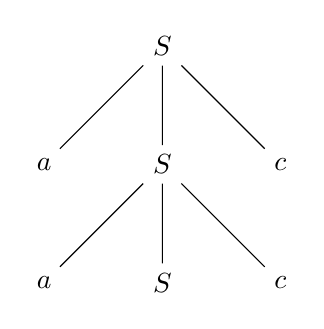
\begin{tikzpicture}
\node{$S$}   
    child {node {$a$}}
    child {node {$S$}
        child {node {$a$}}
        child {node {$S$}}
        child {node {$c$}}}
    child {node {$c$}};
\end{tikzpicture}
\caption{LL(1) Derivation Step 2}
\end{figure}


\textbf{Step 3} Moving onto the next symbol $aa\underline{b}bcc$, we can see that the only production rule which produces a $b$ is $S \rightarrow aSc$ therefore we have to use that one. 

\begin{figure}[H]
\centering
\begin{tikzpicture}
\node{$S$}   
    child {node {$a$}}
    child {node {$S$}
        child {node {$a$}}
        child {node {$S$}
            child {node {$b$}}}
        child {node {$c$}}}
    child {node {$c$}};
\end{tikzpicture}
\caption{LL(1) Derivation Step 3}
\end{figure}

This is the completed parse tree, and as we've seen - we could select the production to use by looking only at the current symbol.
\end{example}

\begin{example}{LL(2) Derivation}
We can take the grammar $S \rightarrow AB$, $A \rightarrow aA\ |\ a$, $B \rightarrow bB\ |\ c$ with the initial non-terminal $S$ for the language $\{a^mb^nc, m \geq 1, n \geq 0\}$ as an example of a LL(2) grammar.

This is a LL(2) grammar because two productions begin with $a$ and we can't determine which one to use without looking ahead to the next symbol. Looking ahead to the next symbol is enough so this must be a LL(2) grammar.

If we take the string $aabbc$, we can see how the LL(2) derivation works. 

\textbf{Step 1} The derivation must begin with $S \rightarrow AB$.

\begin{figure}[H]
\centering
\begin{tikzpicture}
\node{$S$}   
    child {node {$A$}}
    child {node {$B$}};
\end{tikzpicture}
\caption{LL(2) Derivation Step 1}
\end{figure}

\textbf{Step 2} We now take the input string $\underline{a}abbc$ and have a decision to make: use the production $A \rightarrow aA$ or $A \rightarrow a$. To answer this dilemma, we look at the second character of the input string, and as that's an $a$ - we know to use the production which allows for multiple $a$s.

\begin{figure}[H]
\centering
\begin{tikzpicture}
\node{$S$}   
    child {node {$A$}
        child {node {$a$}}
        child {node {$A$}}}
    child {node {$B$}};
\end{tikzpicture}
\caption{LL(2) Derivation Step 2}
\end{figure}

\textbf{Step 3} We now take the second input character $a\underline{a}bbc$ and as that is followed by a $b$ - we know it must be produced with $A \rightarrow a$.

\begin{figure}[H]
\centering
\begin{tikzpicture}
\node{$S$}   
    child {node {$A$}
        child {node {$a$}}
        child {node {$A$}
            child {node {$a$}}}}
    child {node {$B$}};
\end{tikzpicture}
\caption{LL(2) Derivation Step 3}
\end{figure}

\textbf{Step 4} We take the next input character $aa\underline{b}bc$ and as this is followed by another $b$, we know it must be produced with $B \rightarrow bB$. 

\begin{figure}[H]
\centering
\begin{tikzpicture}[level 1/.style={sibling distance=3cm}, level 2/.style={sibling distance=2cm}]
\node{$S$}   
    child {node {$A$}
        child {node {$a$}}
        child {node {$A$}
            child {node {$a$}}}}
    child {node {$B$}
        child {node {$b$}}
        child {node {$B$}}};
\end{tikzpicture}
\caption{LL(2) Derivation Step 4}
\end{figure}

\textbf{Step 5} We take the next input character $aab\underline{b}c$ and as this is followed by a $c$, which we know we can produce from a $B$, so we know the character must be produced with $B \rightarrow bB$.

\begin{figure}[H]
\centering
\begin{tikzpicture}[level 1/.style={sibling distance=3cm}, level 2/.style={sibling distance=2cm}]
\node{$S$}   
    child {node {$A$}
        child {node {$a$}}
        child {node {$A$}
            child {node {$a$}}}}
    child {node {$B$}
        child {node {$b$}}
        child {node {$B$}
            child {node {$b$}}
            child {node {$B$}}}};
\end{tikzpicture}
\caption{LL(2) Derivation Step 5}
\end{figure}

\textbf{Step 6} We take the final input character $aabb\underline{c}$. This isn't followed by anything so we find the production rule which produces this $B \rightarrow c$.

\begin{figure}[H]
\centering
\begin{tikzpicture}[level 1/.style={sibling distance=3cm}, level 2/.style={sibling distance=2cm}]
\node{$S$}   
    child {node {$A$}
        child {node {$a$}}
        child {node {$A$}
            child {node {$a$}}}}
    child {node {$B$}
        child {node {$b$}}
        child {node {$B$}
            child {node {$b$}}
            child {node {$B$}
                child {node {$c$}}}}};
\end{tikzpicture}
\caption{LL(2) Derivation Step 6}
\end{figure}

\end{example}

There are, of course, grammars which don't conform to the LL(k) structure. For example the language $L=\{ba^n, n \geq 0\}$ where the production rules are of the form $S \rightarrow Sa\ |\ b$ is an example of a non-LL(k) grammar. We can show this with the example string $baaaa$. We cannot know precisely how $b$ was derived without knowing the length of the full string; it is impossible to do a partial derivation knowing only how the string starts. 

\subsection{LR(k) Grammars}
The languages based on LR(k) grammars can be parsed bottom up. 

The L in LR(k) means that we scan the string from left to right, however the R means we produce a right-most derivation (R) in reverse. This involves reversing the productions and more more difficult to see through.

LR(1) languages are exactly LR(k) languages which are exactly deterministic context-free languages (DFCL).

Deterministic context-free grammars (DCFG) are a proper subset of the context-free grammars - they can be recognises by the DPDA. DCFGs are always unambiguous.DCFGs are of great practical interest - they cna be parsed in linear time and in fact a parser can be automatically generated from the grammar by a parser generator. 

\begin{example}{LR(0) Grammars}
If we consider the language $L = \{ab^{2n+1}c | n \geq 0\}$ with the grammar $S \rightarrow aAc$ and $A \rightarrow Abb\ |\ b$. We can take the input string $abbbbbc$

To parse this, we we would start at the bottom and work up. We look for the right hand side of the a production in a the string. The first one we find is $b$, which we replace with $A$:
\[a\underline{b}bbbbc \Leftarrow a\underline{A}bbbbc\]

We repeat the process with this new string, and the first one we find is $Abb$:
\[a\underline{Abb}bbc \Leftarrow a\underline{A}bbc\]

We repeat the process on the new string, we again find $Abb$:
\[a\underline{Abb}c \Leftarrow a\underline{A}c\]

Then finally we see $aAc$ which we can produce $S$ from:
\[a\underline{A}c \Leftarrow \underline{S}\]

We can then invert this to find the full derivation from Start Symbol to string of terminals

\[S \Rightarrow aSc \Rightarrow aAbbc \Rightarrow aAbbbbc \Rightarrow abbbbbc\]
\end{example}
